\documentclass[conference]{IEEEtran}
\IEEEoverridecommandlockouts

\usepackage{cite}
\usepackage{amsmath,amssymb,amsfonts}
\usepackage{algorithm}
\usepackage[noend]{algpseudocode}
\usepackage{xcolor}
\usepackage{graphicx}
\usepackage{textcomp}
\usepackage{xcolor}

\def\BibTeX{{\rm B\kern-.05em{\sc i\kern-.025em b}\kern-.08em
    T\kern-.1667em\lower.7ex\hbox{E}\kern-.125emX}}
\makeatletter
\newcommand{\linebreakand}{
  \end{@IEEEauthorhalign}
  \hfill\mbox{}\par
  \mbox{}\hfill\begin{@IEEEauthorhalign}
}
\makeatother
\pagecolor{white}

\begin{document}

\title{Petification: Node-RED based Pet Care IoT Solution \\ using MQTT Broker}

\author{
    \IEEEauthorblockN{Haeram Kim}
    \IEEEauthorblockA{
        \textit{Computer Science and Engineering} \\
        \textit{Chungnam National University}\\
        Daejeon, Korea \\
        haeram.kim1@gmail.com
    }
    \and
    \IEEEauthorblockN{Hyejong Kang}
    \IEEEauthorblockA{
        \textit{Computer Science and Engineering} \\
        \textit{Chungnam National University}\\
        Daejeon, Korea \\
        kanghyejong1001@gmail.com
    }
    \and
    \IEEEauthorblockN{Sunghan Kim}
        \IEEEauthorblockA{
        \textit{Computer Science and Engineering} \\
        \textit{Chungnam National University}\\
        Daejeon, Korea \\
        seonghan.kim.cnu@gmail.com
    }
    \linebreakand
    \IEEEauthorblockN{Dukho Choi}
    \IEEEauthorblockA{
        \textit{International trade / software convergence} \\
        \textit{Chungnam National University}\\
        Daejeon, Korea \\
        dukho.fin@gmail.com
    }
    \and
    \IEEEauthorblockN{Jihyun You}
    \IEEEauthorblockA{
        \textit{Cybersecurity} \\
        \textit{Purdue University}\\
        West Lafayette, IN, USA \\
        you62@purdue.edu
    }
}

\maketitle 

\begin{abstract}
While there are an increasing number of households owning pets, it is challenging for owners who leave home often to take good care of their pets.
However, most previous studies regarding remote food/water serving use limited featured IoT platforms, and do not provide any notification or alerts about remaining amount of food/water.
Thus, a novel IoT solution "Petification" is proposed, which uses an open-source project Node-RED combined with MQTT messaging protocol to provide information about device connectivity, available resource, and consumption via a web-based dashboard.
Additionally, Petification provides empty notification service and remote feeding service.
The water supplier and feed machine are attached to the platform to provide water and food to the pet and scale the weight of the water and food.
The load cell, HX711 amplifier, and Raspberry Pi Zero W are mounted to the water supplier and feed machine and an MG90S servo motor is mounted to the Raspberry Pi of the feed machine.
However, served amount of the food sometimes mismatches with the desired amount while testing the implementation.
Thus the future plan can be to enhance the food gate to serve the exact amount of food. \\
\end{abstract}

\begin{IEEEkeywords}
IoT platform, Node-RED, MQTT, Smart pet care service 
\end{IEEEkeywords}

\section{Introduction}
% `Project background`
As the number of single-person household increases and the raising pet culture spread compared to the past, the number of households raising pets is increasing.
The growth of the pet industry is a good example showing this trend: Profit of pet industries have doubled every year over 10 years, from \$48.4 billion in 2010 to \$109.6 billion in 2020 \cite{b1}.
Along with this trend, demand for tracking pet wellness is increased accordingly.
For people who leave their house frequently, it is hard to track the pet's status when left alone, and thus demand for a relevant service.

% `Problem statement`
Internet of Things (IoT) has recently received attention for the solution to these challenges.
However, despite the various pet care IoT solutions and studies conducted in the past, most of the used IoT platforms have limitations of not being open-sourced.
For instance, the most commonly used IoT platform such as "blynk" \cite{b2, b3, b4} has stopped supporting open-source versions, and other common platforms such as "Adafruit IO" \cite{b5} and "Freeboard IO" \cite{b6} does not support open-source versions. 
Moreover, while these solutions support tracking food/water consumption and automatic feeding, few support functions such as device status information and error notification.

% `Project novelty`
Thus a novel solution "Petification" which uses open-source projects for the IoT platform, is proposed.
Node-RED which is a flow-based open-source visual programming tool \cite{b7} is used to implement the APIs of the IoT platform.
This allows Petification to be able to develop more faster, provide user-friendly UI to the user, and make use of rich resource ecosystem generated by users. 
To manage overall message flows, Eclipse Mosquitto which is one of the open-source implementations of the MQTT messaging protocol is used.
Using the MQTT protocol as a message broker allows the IoT platform to connect the device to the user in a lightweight way \cite{b8}.

% `Functionality`
Petification provides a wide array of information such as device connectivity, the remaining amount of food/water for each device, and amount of consumption visually with the web-based dashboard.
It also provides an email and "WhatsApp" messanger based error notification service when the water or food is running out, as well as automatic feeding service.
The water supplier and feed machine are attached to the platform to feed and water the pet and to scale the weight of the food/water.
While both the water supplier and feed machine use the load cell to scale the weight, a servo motor is attached only to the feed machine so that the user can control the served amount of food.
All the load cells and a servo motor are mounted to Raspberry Pi for each device.

\section{Related Literature}
% TODO:
%여기는 단순히 XXX가 proposed AAAA 이런 형식을 반복하는것보다는,
%The functionality of AAAA has been widely implemented. XXXX and YYYY implemented AAAA by using....
%BBBB has also received attention by previous work. For instance, XXXX implemented BBBB by using ~~ technique.... 이렇게 흐름을 이어나가는것이 좋지 않을까... 여기는 내가 문헌을 읽지 않았으므로 pass
T. Sangvanloy \textit{et al.} \cite{b3} proposed a pet care IoT solution that visualizes the daily food consumption in real-time and automatically feeds the pet according to the scheduled time.
The conducted research also provides an automatic serving amount adjustment feature based on the pet's species and weight.
The IoT solution was implemented with ESP32 Wi-Fi micro-controller, servo motor, load cell, and “Blynk” IoT platform.

Y. Chen \textit{et al.} \cite{b4} proposed a pet care IoT solution that provides information such as food and water consumption, the number of defecation, and defecation duration.
It was implemented using Arduino Uno and ESP8266 Wi-Fi Module with load cell, servo motor, and motion sensor.
A mobile application is provided to the user with the help of the “Blynk” IoT platform.

P. N. Vrishanka \textit{et al.} \cite{b9} proposed an automated pet feeder which serves food to the pet according to the remaining amount of food in the food bowl.
An ultrasonic distance sensor and SG90 servo motor were mounted to Arduino Uno R3 in this research.
An ultrasonic distance sensor is used to determine the remaining food amount by measuring the distance from the entrance of the feed container to the inside of the bowl.

Rogerio Nogueira \textit{et al.} \cite{b10} proposed a system that can serve food and water according to pre-scheduled times and amounts.
Additionally, the system provides a notification service for abnormal situations with photos and alerts and a "chat-based" intelligent interface to the user.
This research is conducted with Raspberry Pi, Python, Telegram cloud service, and IBM Watson Assistant.

Vania \textit{et al.} \cite{b11} proposed an IoT solution that identifies each pet via RFID and serves food by schedule.
The dog feeder in the research was developed using Arduino Uno and ESP8266 Wi-Fi Module with load cell and DC motor.
An Android mobile application is provided to the user and the IoT platform is developed with Node JS and MySQL database.
Communication between the device and the user is based on MQTT over SSL/TLS protocol.

\section{Methodology}
The system architecture for Petification is designed to connect the feed machine and water supplier with the user.
Each user and device can communicate bi-directionally through the platform.
The feed machine and water supplier are connected to the Access Point (AP) through Wi-Fi.
Thus, all messages published from the device are first sent to the AP through Wi-Fi, and then to the Petification platform through the internet.
The platform processes the messages and sends the processed data to the users in form of a web dashboard page, E-Mail, and WhatsApp messages.
On the contrary, users can send requests to the platform via the web dashboard.
while some requests require only the platform, requests to activate the actuator are sent to the device with the help of the platform.
Figure 1 shows the overview of for Petification.


\begin{figure}[htbp]
\centerline{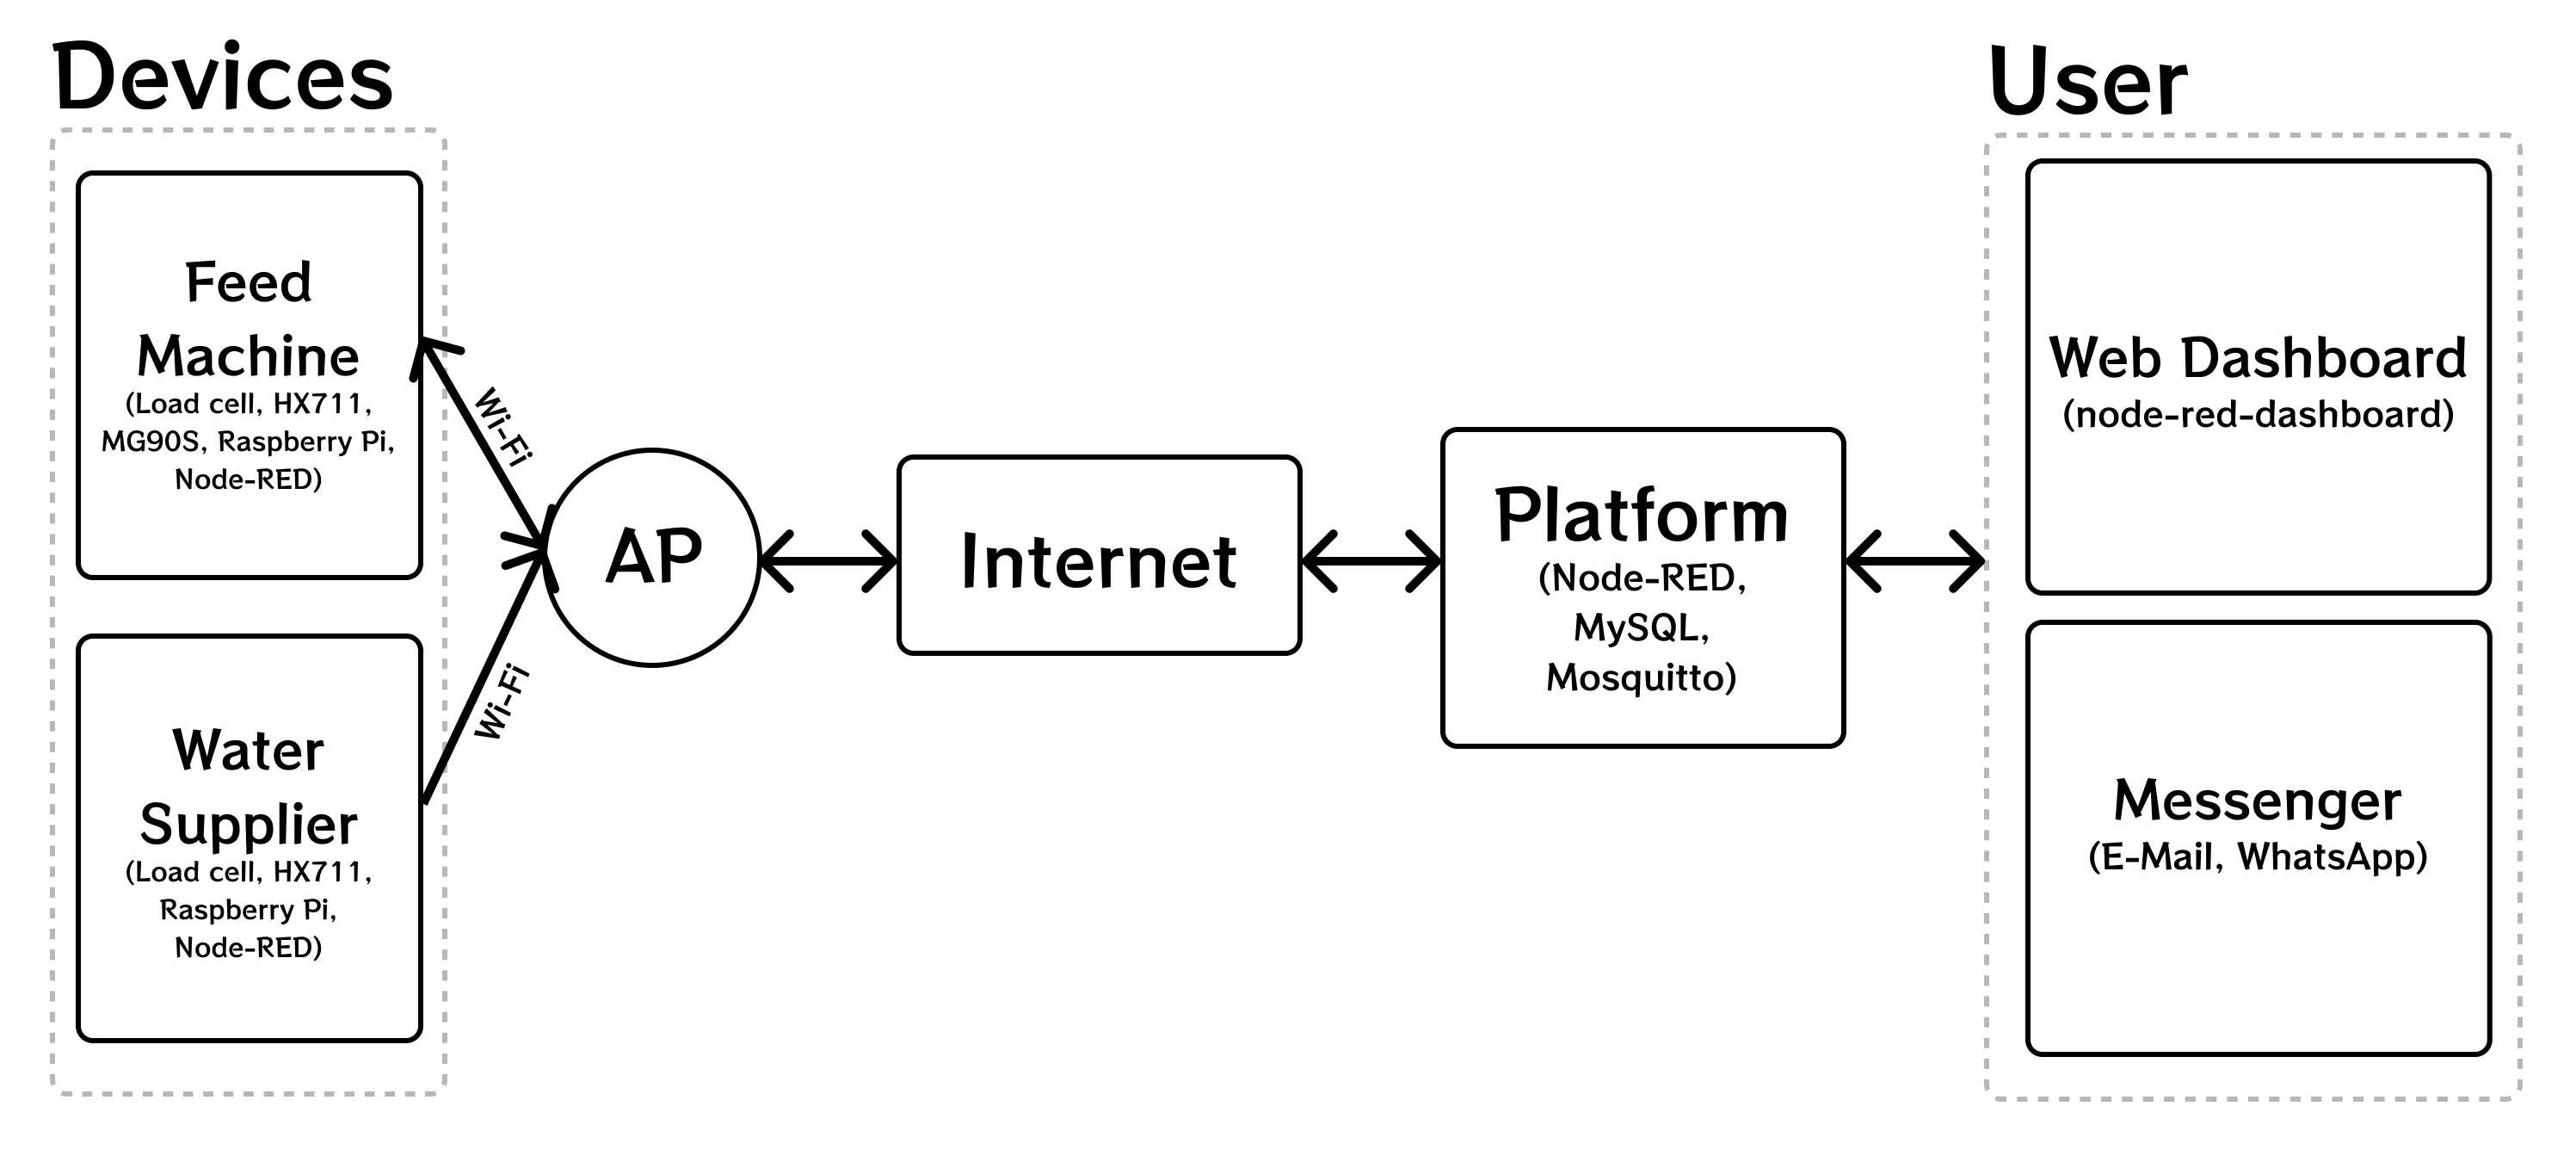
\includegraphics[width=0.5\textwidth]{./images/Overview.png}}
\caption{Petification overview}
\label{fig}
\end{figure}

\subsection{Water Supplier}
Measuring the weight of the water is done with single load cell which scales up to a maximum of 5kg with 1g accuracy.
As shown in figure 3, The load cell is installed between the two plates to measure the pressure applied to an upper plate as shown in figure 2 and is attached to the Raspberry Pi Zero W through the HX711 amplifier which converts the analog signal to the digital signal.
To convert the measurement of the load cell to the weight data, the calibration process has proceeded to get the reference unit.
The formula for calibration is shown below:
\[
   referenceUnit = \frac{average(loadCellMeasurements)}{actualWeight}
\]

A 500mL water bottle which is used as an actual weight of 500g is measured 500 times to get a reference unit in the calibration process.

\begin{figure}[htbp]
\centerline{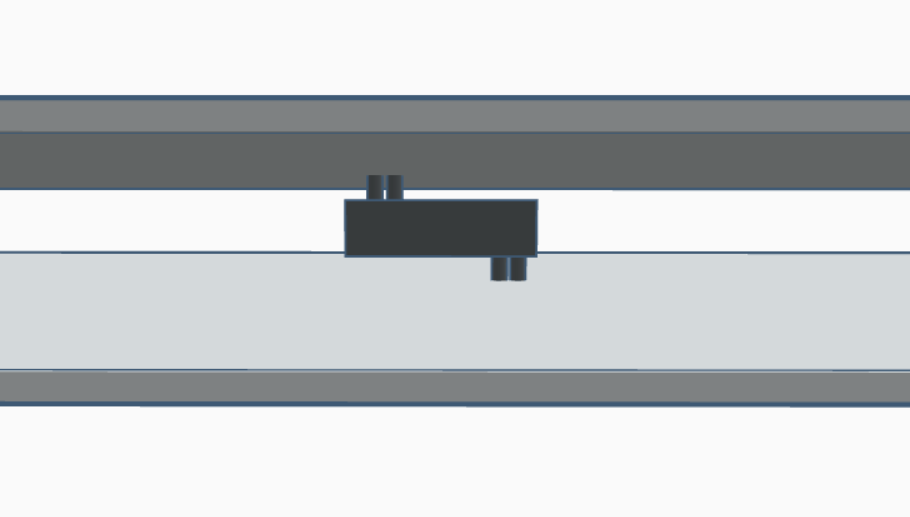
\includegraphics[width=0.3\textwidth]{./images/load-cell.png}}
\caption{Installaion of a load cell}
\label{fig}
\end{figure}

\begin{figure}[htbp]
\centerline{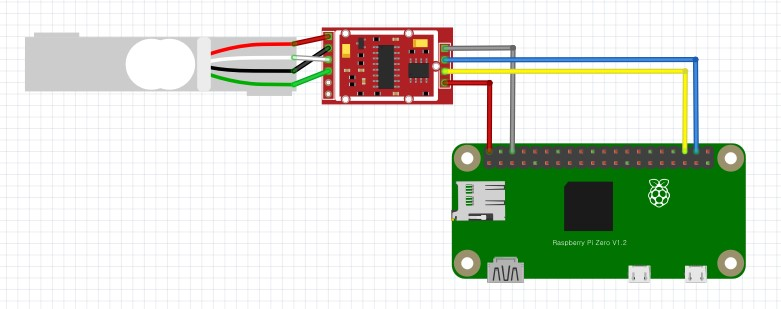
\includegraphics[width=0.5\textwidth]{./images/water supplier circuit.jpg}}
\caption{Circuit diagram of the water supplier}
\label{fig}
\end{figure}

\subsection{Feed Machine}
To serve food to the pet, an MG90S servo motor is mounted to open and close the food gate.
As in figure 4, the servo motor gives food in an open/close type.
Food serving is done with the help of gravity; After the food gate is opened, food rolls down the slope, and thus food is served.
By closing the food gate Feed Machine stops the serving of the food.
Two load cells and two HX711 amplifiers are installed in the same way as the water supplier under the food bowl and container to measure the weight of the food.
All the load cells, HX711 amplifiers, and an MG90S servo motor are attached to the Raspberry Pi Zero W as shown in figure 5.

\begin{figure}[htbp]
\centerline{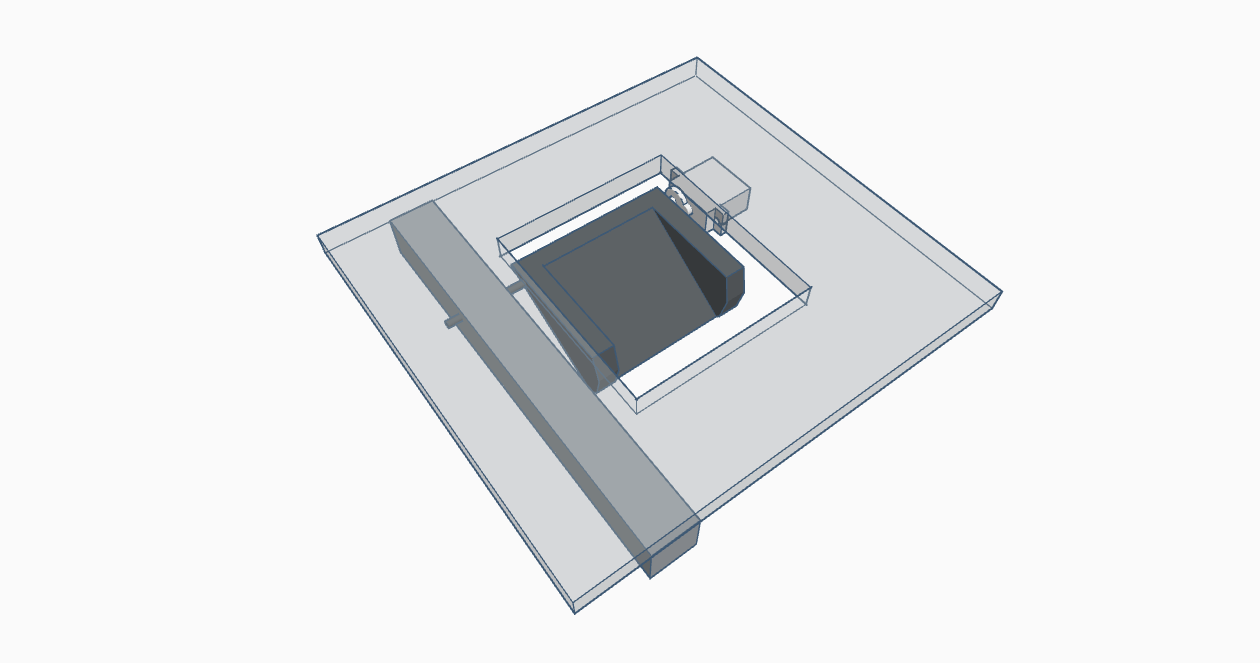
\includegraphics[width=0.5\textwidth]{./images/servo_gate.png}}
\caption{Food gate of the feed machine}
\label{fig}
\end{figure}

\begin{figure}[htbp]
\centerline{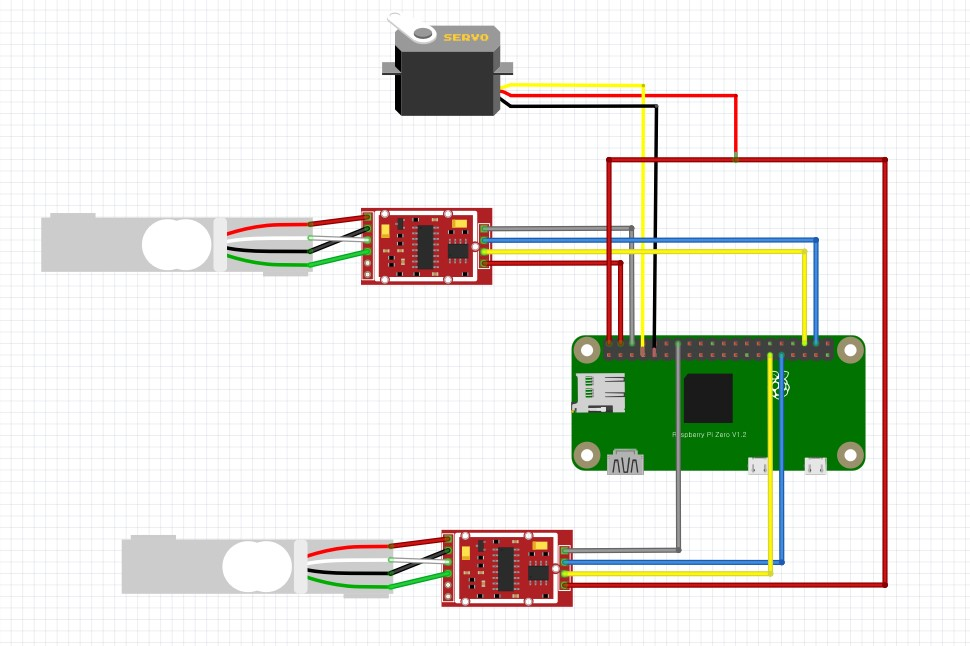
\includegraphics[width=0.5\textwidth]{./images/feed machine circuit.jpg}}
\caption{Circuit diagram of the feed machine}
\label{fig}
\end{figure}

\subsection{IoT Platform}
The user-to-device communication occurred when the user wants to serve the food to the pet, and device-to-user communication occurred to provide information and notification to the user.
To serve the food, the user can either set the serving schedule or press the button in the dashboard.
The serving schedules are stored in the database and checked every minute to send the message to the feed machine when the scheduled time arrives.
The food serving message is also sent when the user presses the button.
After the feed machine receives the message, it opens the food gate and scales the food bowl repeatedly to serve the desired amount of food to the pet.
The detailed flow for the food serving is shown in figure 6.

\begin{figure}[htbp]
\centerline{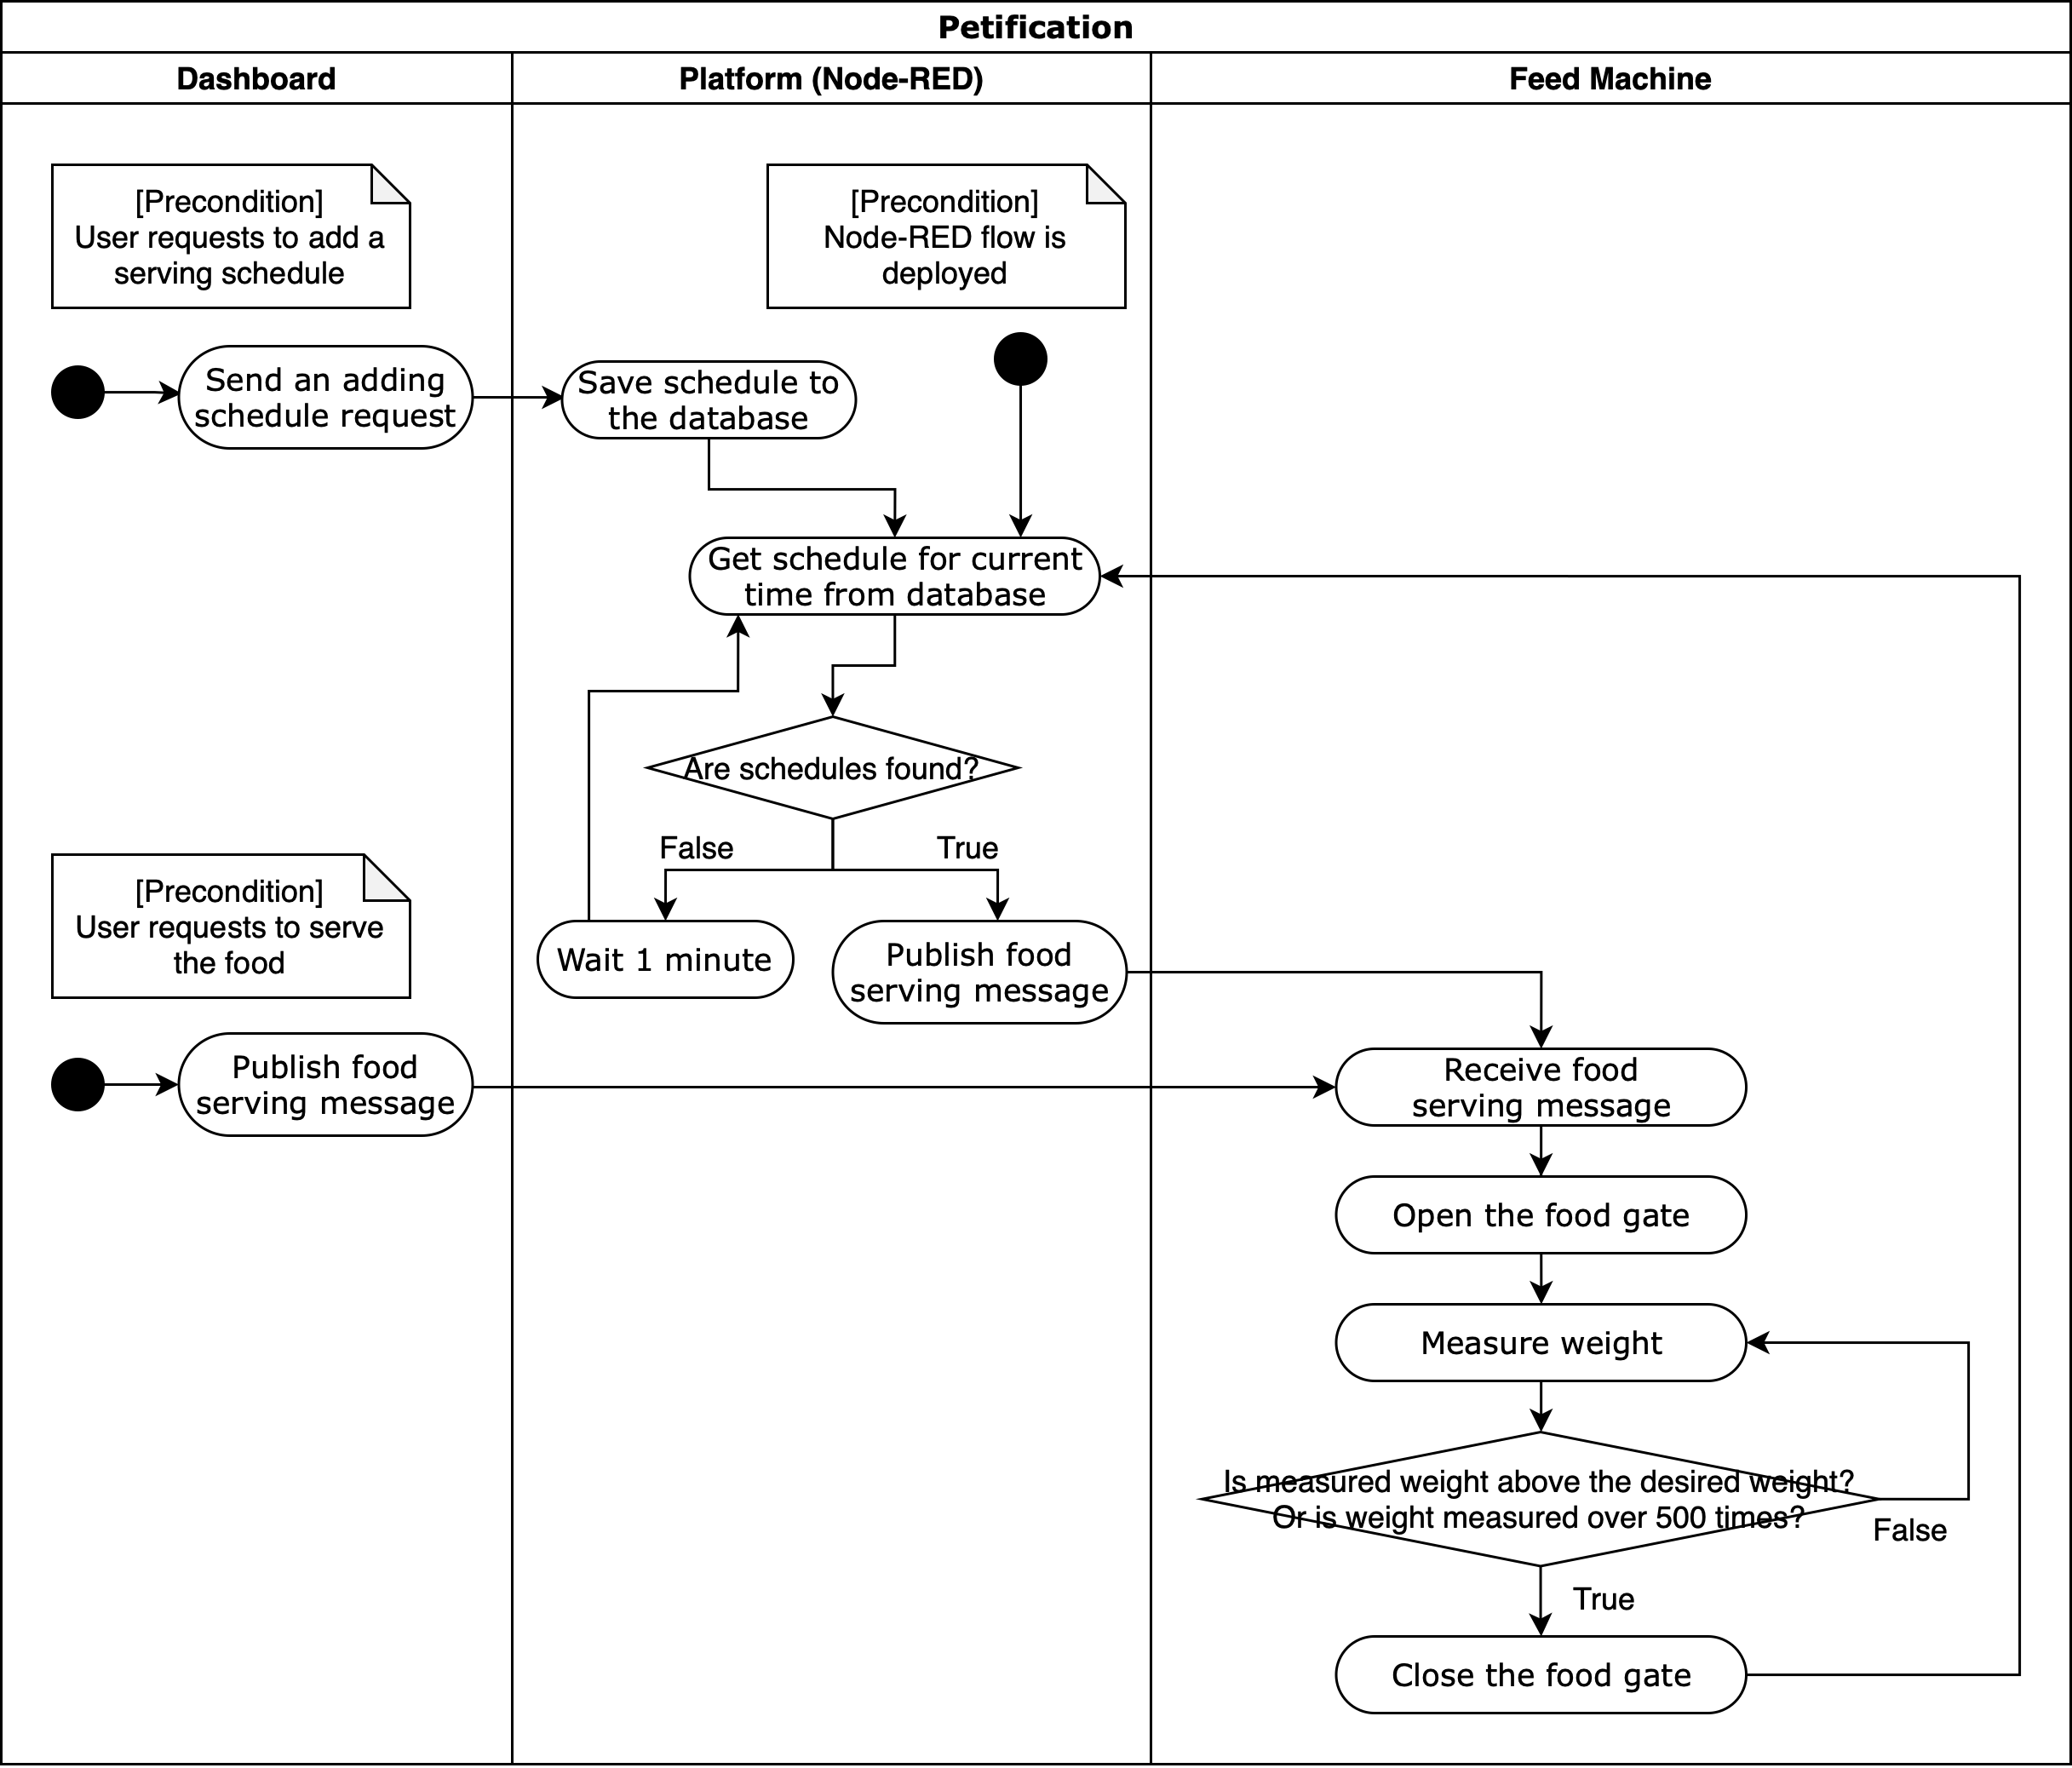
\includegraphics[width=0.5\textwidth]{./images/user2device.png}}
\caption{Activity diagram for user-to-device communication}
\label{fig}
\end{figure}

To provide information and notification to the user, both the water supplier and feed machine scale what they stores.
When the measured weight is above a certain threshold, they send a message containing the measured weight to the platform.
This data message is used to update and show the remaining amount, consumption, and device status to the user.
However, when the measured weight is below the threshold, then an error message is sent to the platform to update the device status and to notify the user that the food/water is empty.
The detailed device-to-user flow is shown in figure 7 and the pseudo-code for calculating the consumption is shown in algorithm 1.

\begin{figure}[htbp]
\centerline{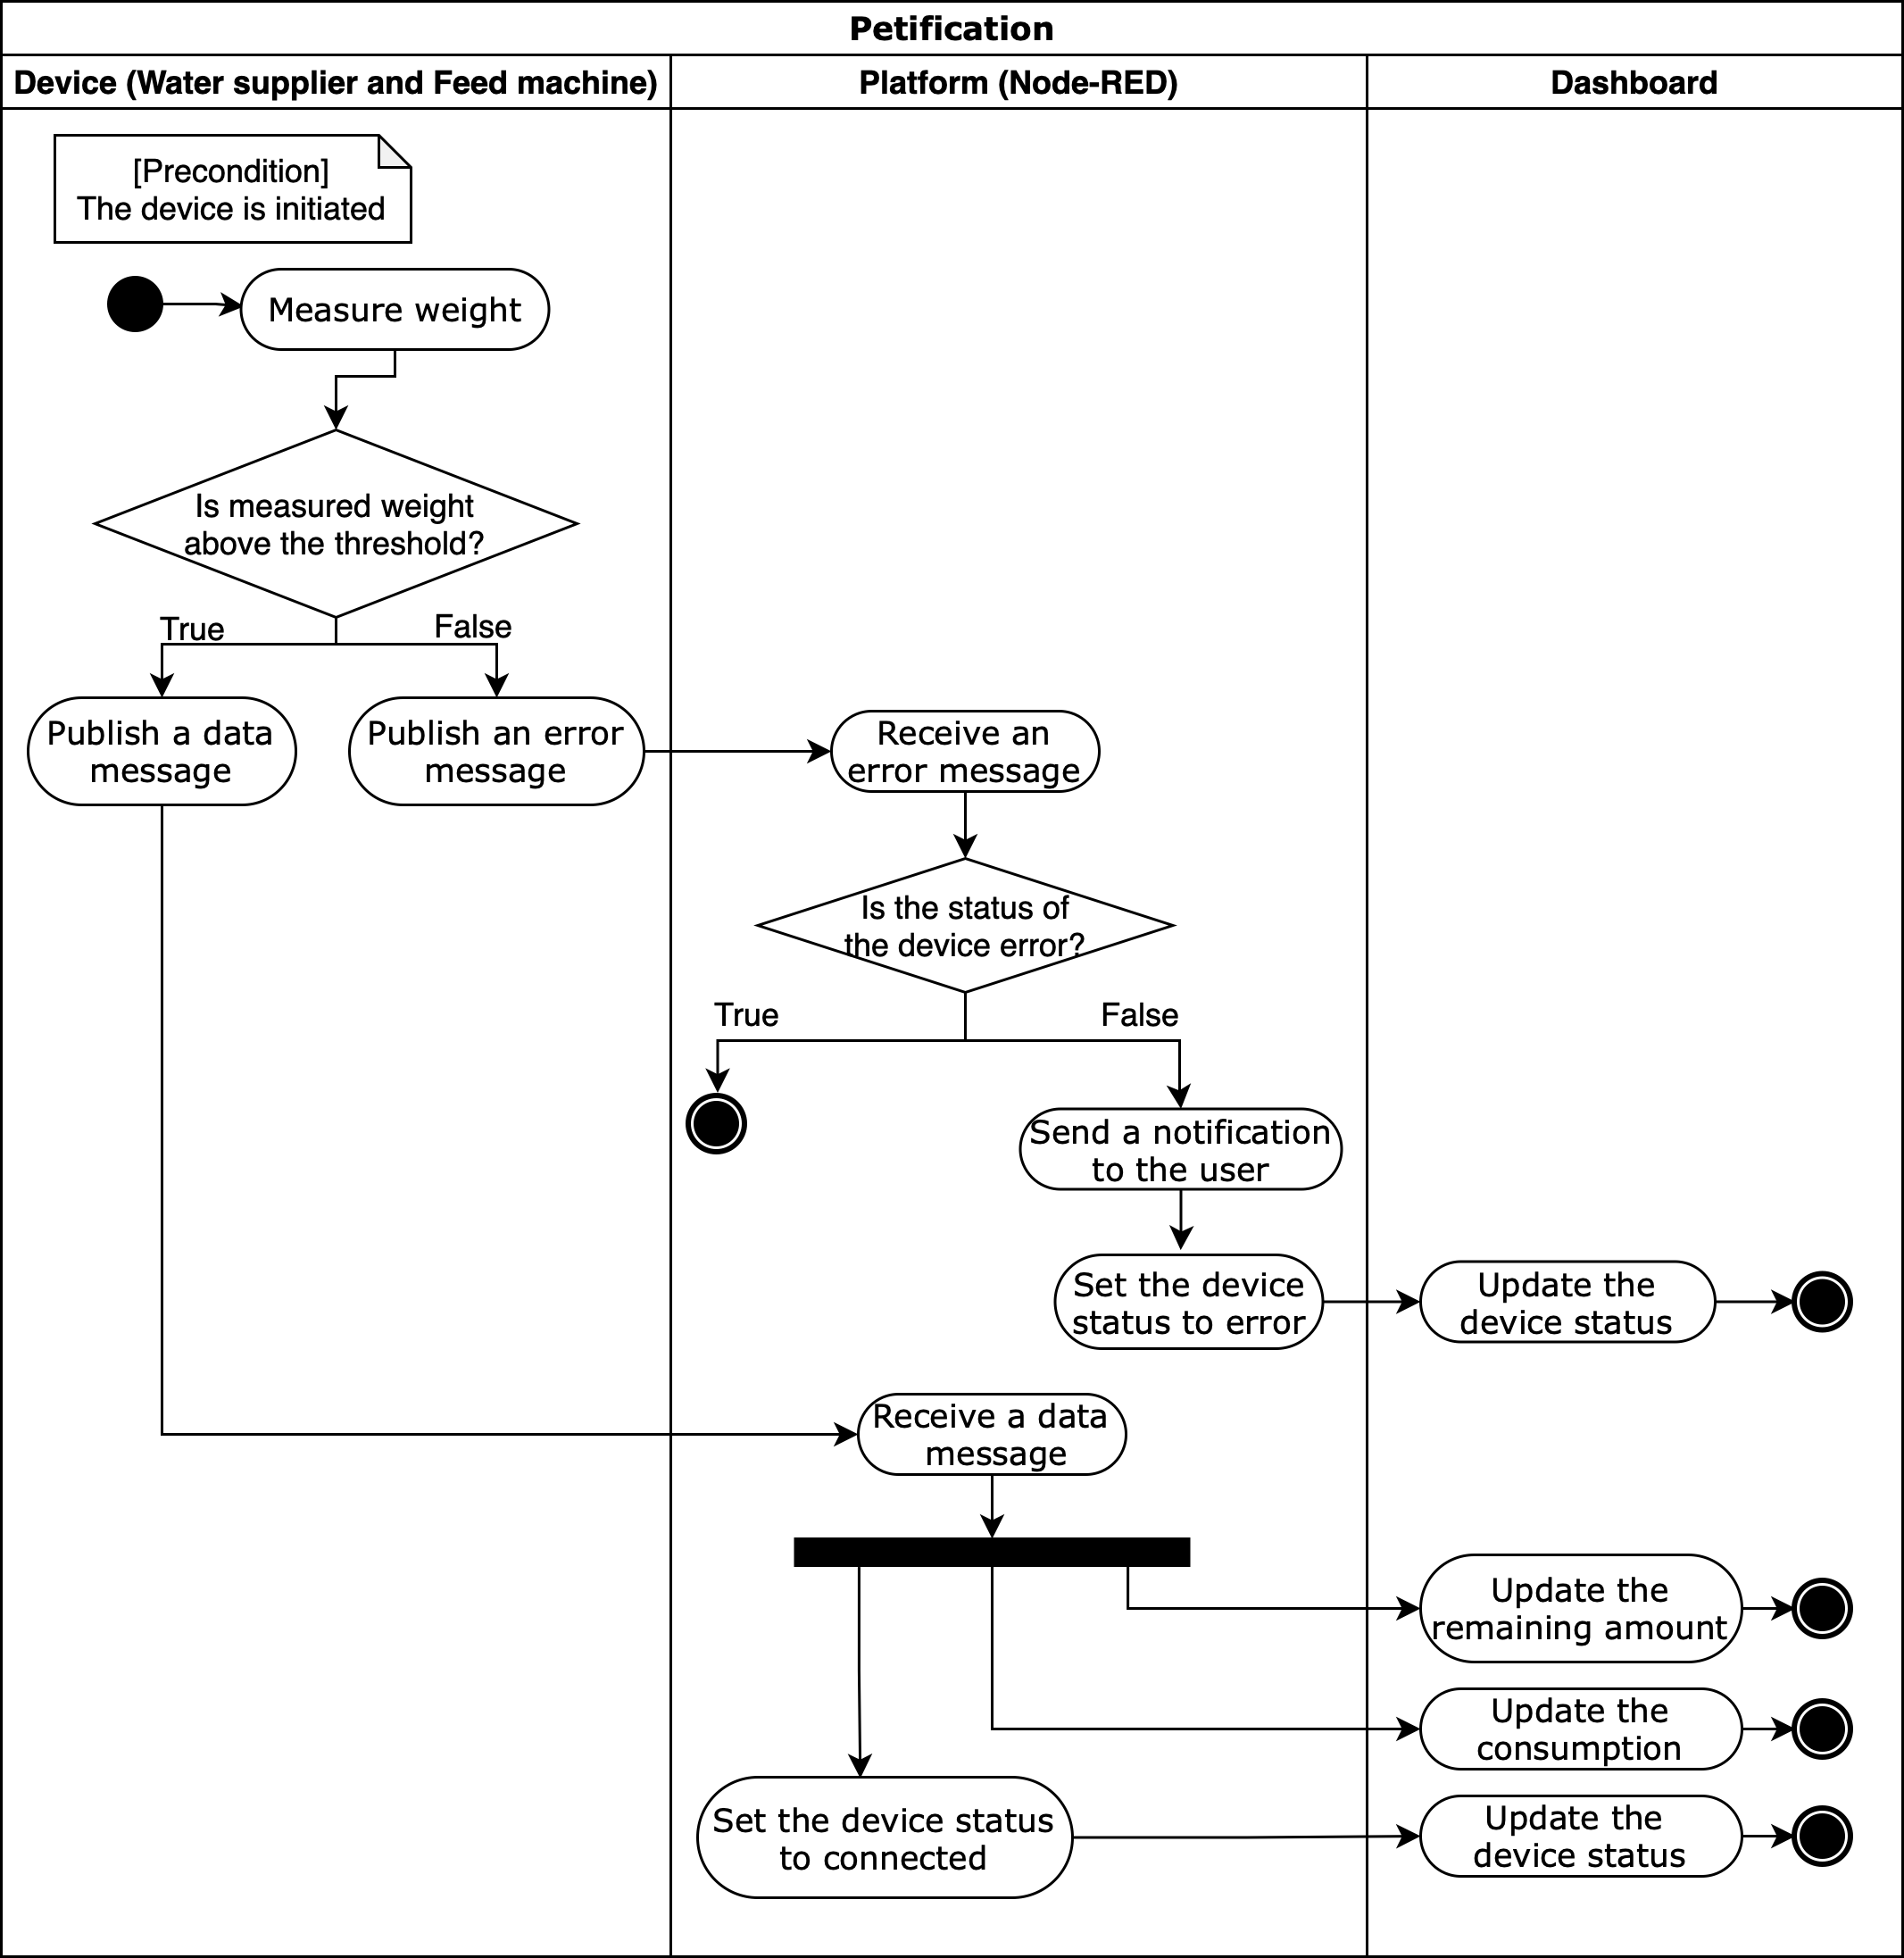
\includegraphics[width=0.5\textwidth]{./images/device2user.png}}
\caption{Activity diagram for device-to-user communication}
\label{fig}
\end{figure}

\begin{algorithm}
\caption{Calculate consumption}\label{algo}
\begin{algorithmic}[1]
    \Procedure{CalcConsumption}{}
        \State $prevConsumption \gets \text{previous } \textit{consumption}$
        \State $currScale \gets \textit{scale} \text{ of received message}$
        \State $prevScale \gets \textit{scale} \text{ of  previous record}$
        \State $decrease \gets 0$
        \If{$precScale \neq \textit{null} \And prevScale > currScale$}
            \State $decrease \gets prevScale - currScale$
        \EndIf
        \Return $prevConsumption + decrease$
    \EndProcedure
\end{algorithmic}
\end{algorithm}

Three open-source projects are used in the platform: Node-RED, Eclipse Mosquito, and MySQL.

\subsubsection{Node-RED}
Node-RED is a flow-based open-source visual development tool that is easy for developers and non-developers to develop programs \cite{b12}.
One of the strengths of the Node-RED is its powerful community.
Not only Node-RED itself but also various nodes such as dashboard widgets and database drivers are being distributed through Node Package Manager (NPM).
Another strength is that it can run on various environments such as local, Raspberry Pi, Docker, and Cloud Instance.
Thus, Node-RED v2.2.1 is installed in not only the platform server but also Raspberry Pi of water supplier and feed machine.

\subsubsection{Eclipse Mosquitto MQTT message broker}
MQTT (Message Queuing Telemetry Transport) is an OASIS standard protocol and provides lightweight, publish/subscribe messaging transport for IoT \cite{b8}.
The publish/subscribe model of the MQTT protocol allows the IoT platform to support bi-directional communication in a way that one can subscribe to the "topic" of the message to receive a message published to that "topic" by another.
In this research, Eclipse Mosquitto v1.4.15 is used as an MQTT Message Broker.
Eclipse Mosquitto is an open-source message broker implementing MQTT protocol versions 5.0, 3.1.1, and 3.1 \cite{b13}.

\subsubsection{MySQL}
MySQL is a fast, flexible, and easy-to-use open-source database with RDBMS (relational database management system).
In addition to the performance and security perspectives, MySQL is considered a suitable database to manage effective data flows because it has good compatibility with Node-RED.
For this reason, MySQL v5.7.37 is integrated as a component of the platform.

\section{Implementation}
\subsection{Water supplier}
Calibrating and measuring the weight of the water is done with python code.
By using the "exec" node of the Node-RED to execute python code, the result of a measurement can be used in Node-RED.
However, even if the calibration has proceeded, there is always the possibility of measurement error.
Thus the "smooth" node of the "node-red-node-smooth" node module has been used to get a maximum value of two measurement results.
After the weight is measured, the "switch" node determines what type of message (weight data or error) has to be sent by checking if the weight is below the threshold value which is 10g for this implementation.
The messages are sent after the "function" node prepares the message and the "mqtt out" node publishes the message.
The Node-RED flow for publishing weight or error messages is shown in figure 8 and the implemented water supplier is shown in figure 9.

\begin{figure}[htbp]
\centerline{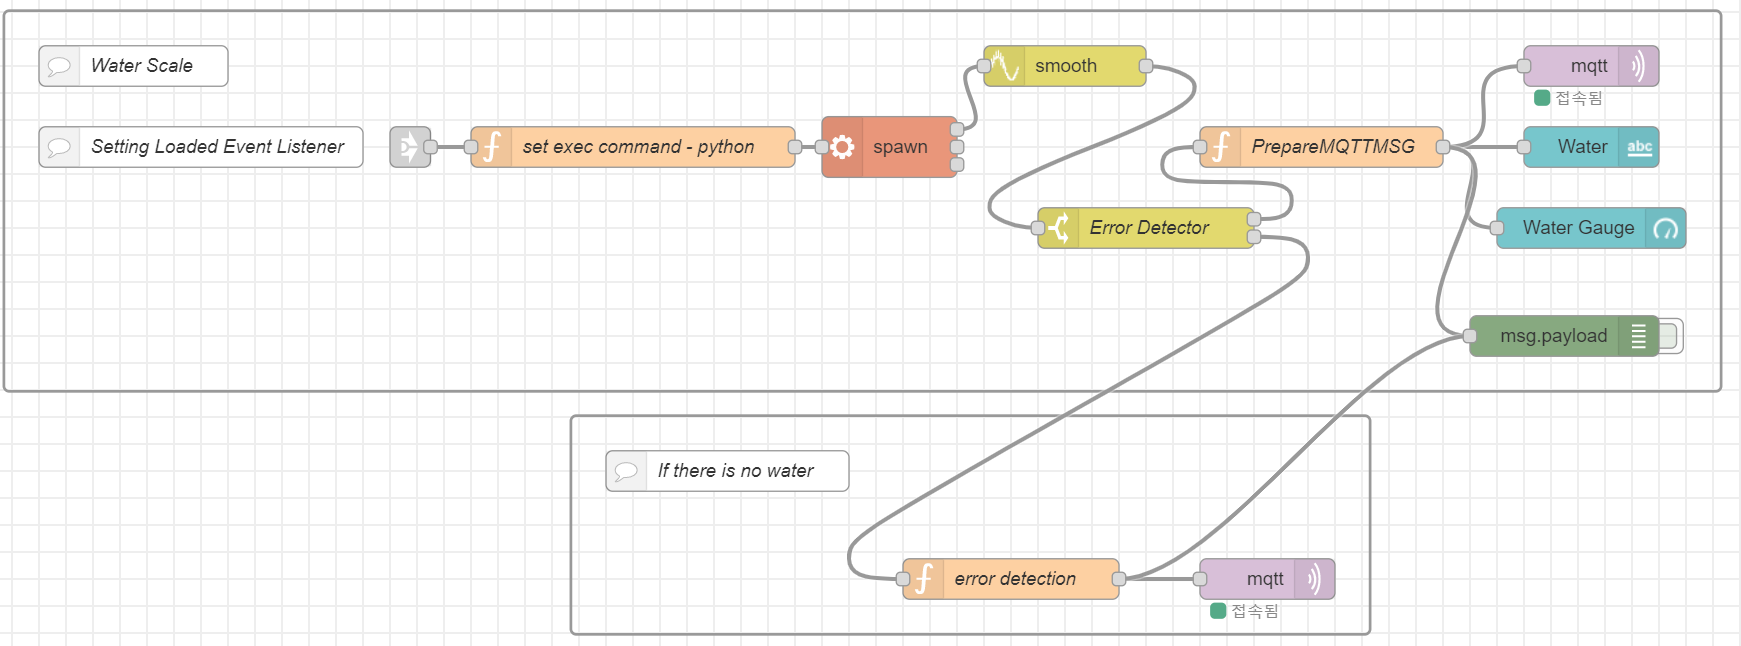
\includegraphics[width=0.5\textwidth]{./images/Water Supplier Error Detection.png}}
\caption{Node-RED screenshot for publishing weight or error message}
\label{fig}
\end{figure}

\begin{figure}[htbp]
\centerline{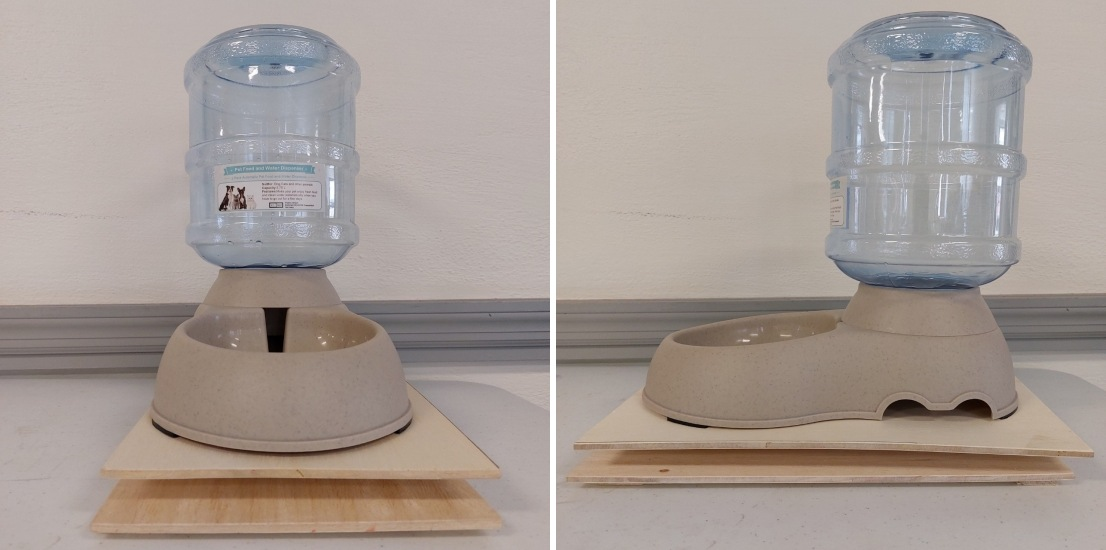
\includegraphics[width=0.5\textwidth]{./images/water-supplier.jpg}}
\caption{Result of implementation for water supplier}
\label{fig}
\end{figure}

\subsection{Feed machine}
In addition to the weight measuring flow which is the same as that of the water supplier, the flow for serving a certain amount of the food to the pet is implemented in the feed machine.
Food serving flow does not begin before a message which contains desired serving amount at the message payload arrives.
The "join-wait" node of the "node-red-contrib-join-wait" node module waits for a food serving message and returns an object which contains a current weight for that time and desired weight after the serving message has arrived.
Then, the current weight is measured and compared repeatedly by a "loop" node of the "node-red-contrib-loop-processing" and a "change" node.
The food gate is opened for the first loop and is closed when the current weight is above the desired weight or the loop is repeated 500 times by the "pi-gpiod out" node of the "node-red-node-pi-gpiod" node module.
The Node-RED flow for serving food is shown in figure 10 and the implemented feed machine is shown in figure 11.

\begin{figure}[htbp]
\centerline{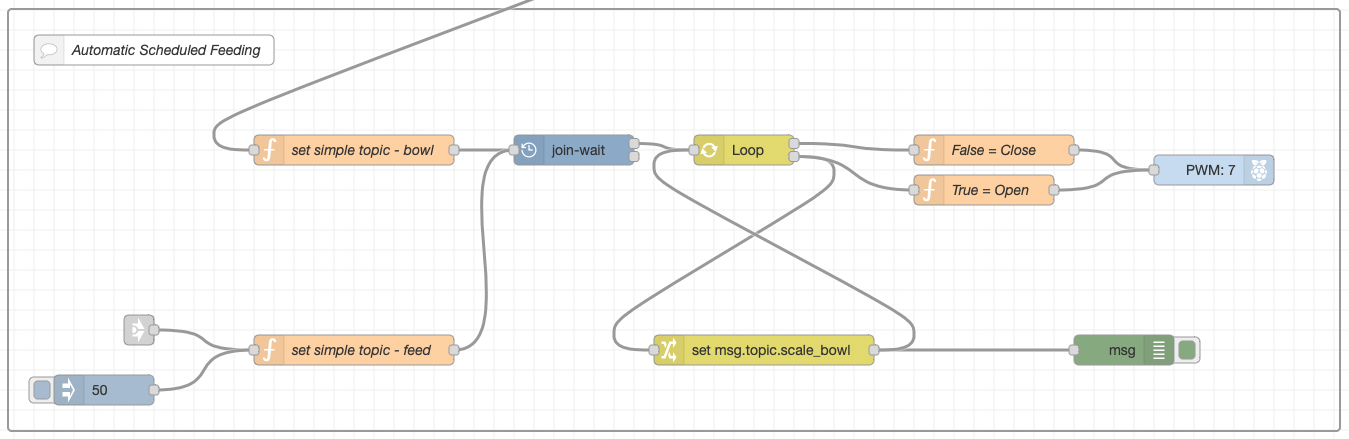
\includegraphics[width=0.5\textwidth]{./images/automaticFeeding.png}}
\caption{Node-RED screenshot for automatic feeding}
\label{fig}
\end{figure}

\begin{figure}[htbp]
\centerline{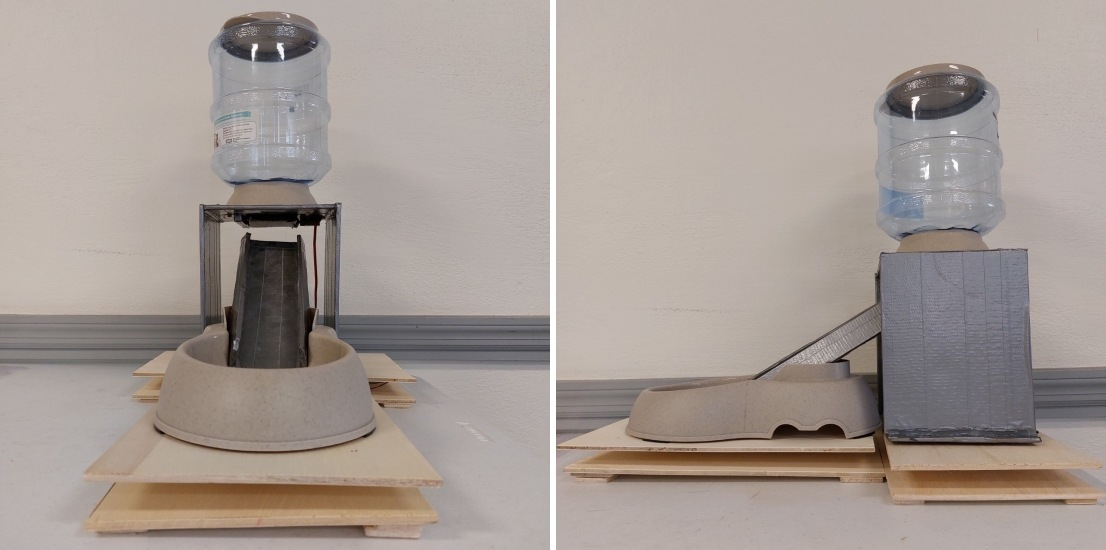
\includegraphics[width=0.5\textwidth]{./images/feed-machine.jpg}}
\caption{Result of implementation for feed machine}
\label{fig}
\end{figure}

\subsection{IoT Platform}
The platform for Petification uses cloud instances for deployment.
On the cloud instance, Eclipse Mosquitto, MySQL, and Node-RED are installed and the firewall, DNS, and certificate for TLS/SSL communication are configured for networking.
In the Node-RED, 7 IoT platform components are implemented as 7 flows.
A screenshot for implemented Node-RED flows is shown in Figure 12.

\begin{figure}[htbp]
\centerline{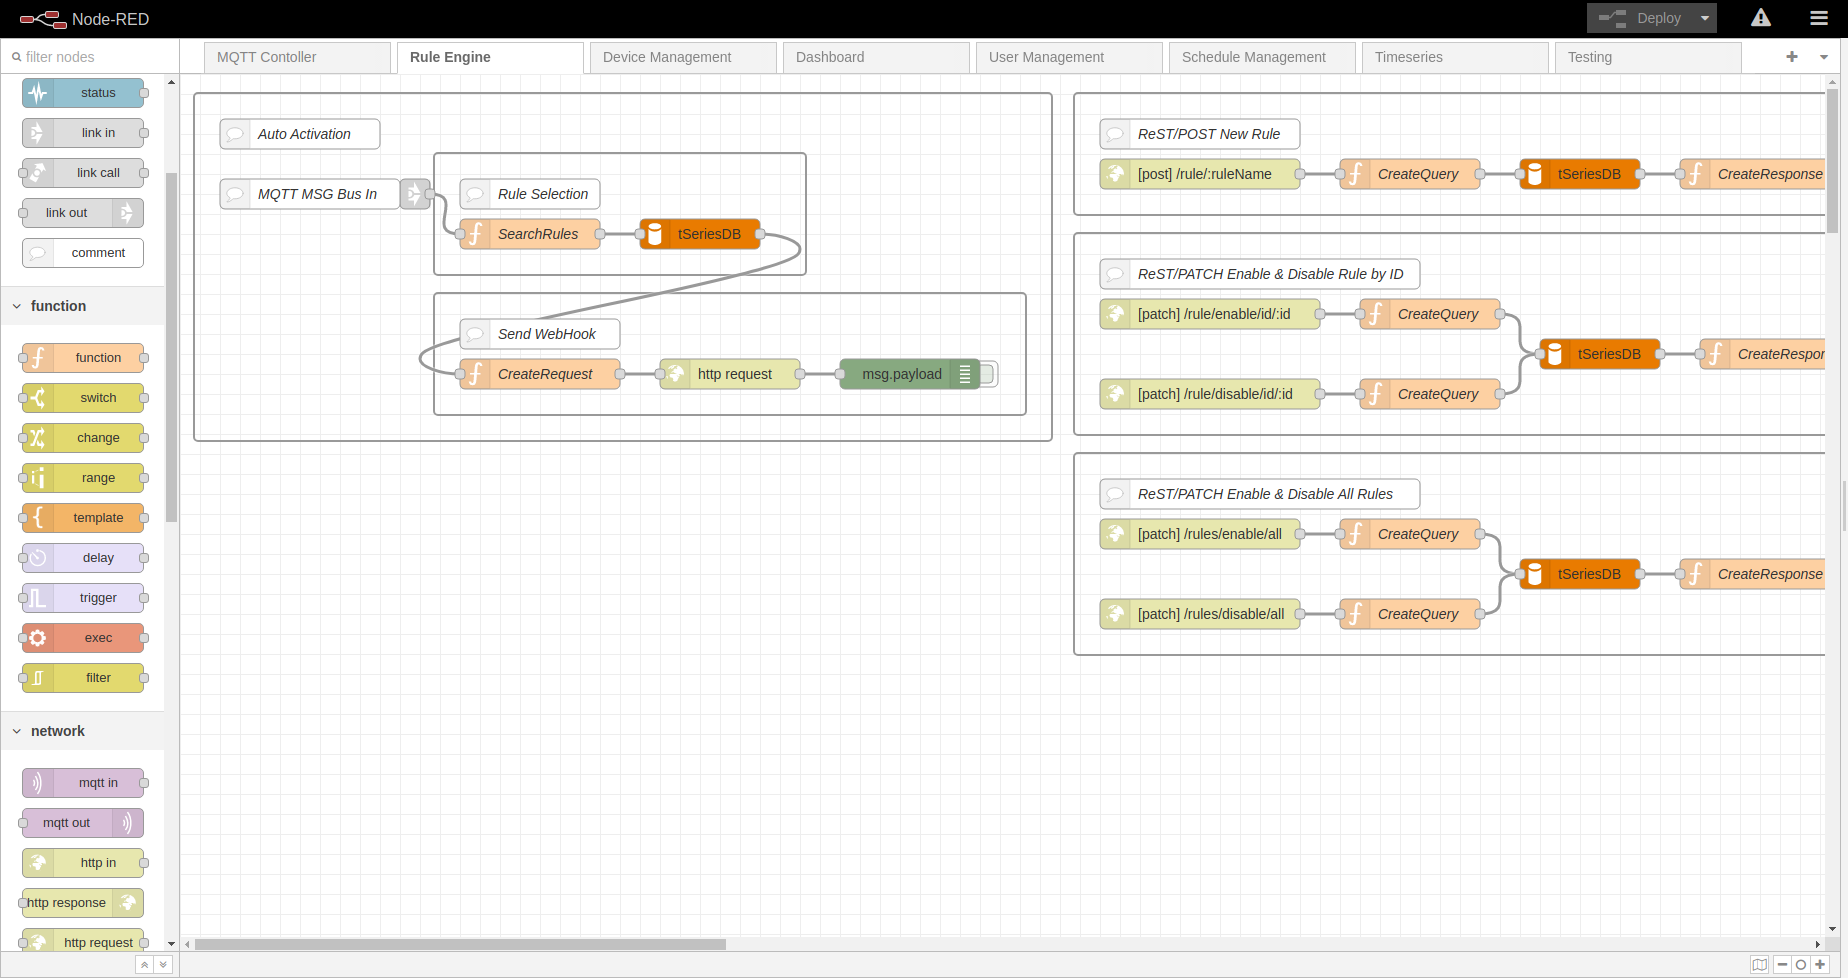
\includegraphics[width=0.5\textwidth]{./images/node-red-platform-screenshot.png}}
\caption{Node-RED flow screenshot of IoT platform}
\label{fig}
\end{figure}

\subsubsection{MQTT Controller}
MQTT Controller flow in the Node-RED is the gateway for MQTT messages to enter Node-RED.
The main purpose of this flow is to parse the topic and payload of the incoming MQTT message to provide useful information such as the MQTT username and client id to other flows.
The "mqtt in" node is used to subscribe and receive the MQTT message and the "function" node is used to parse the message and convert it to an object.

\subsubsection{Rule Engine}
The purpose of Rule Engine is to activate actions according to MQTT messages.
Designing logic of the Rule Engine is inspired by the book, “Build Your Own IoT Platform” \cite{b14}.
For every published message, Rule Engine searches for all rules where the rule’s message pattern satisfies the message content.
Actions that corresponded to the rules are defined as ReST API form, thus activating action will be progressed as sending an HTTP request.

\subsubsection{Device Manager}
Handling devices that are attached to the platform is the main purpose of the Device Manager flow.
It provides ReST APIs that can add a new device to the platform, modify the status of the device, and delete a device.
And it also provides functionality for publishing an action-type message to a specific device.

\subsubsection{Dashboard}
Dashboard Manager is to provide a Graphical User Interface (GUI) to the user.
By using this flow, users can be provided the status of water and food remaining and consumption visually.
It also provides buttons to serve food and input areas to set user settings. A screenshot of the implemented dashboard is shown in figure 13.

\begin{figure}[htbp]
\centerline{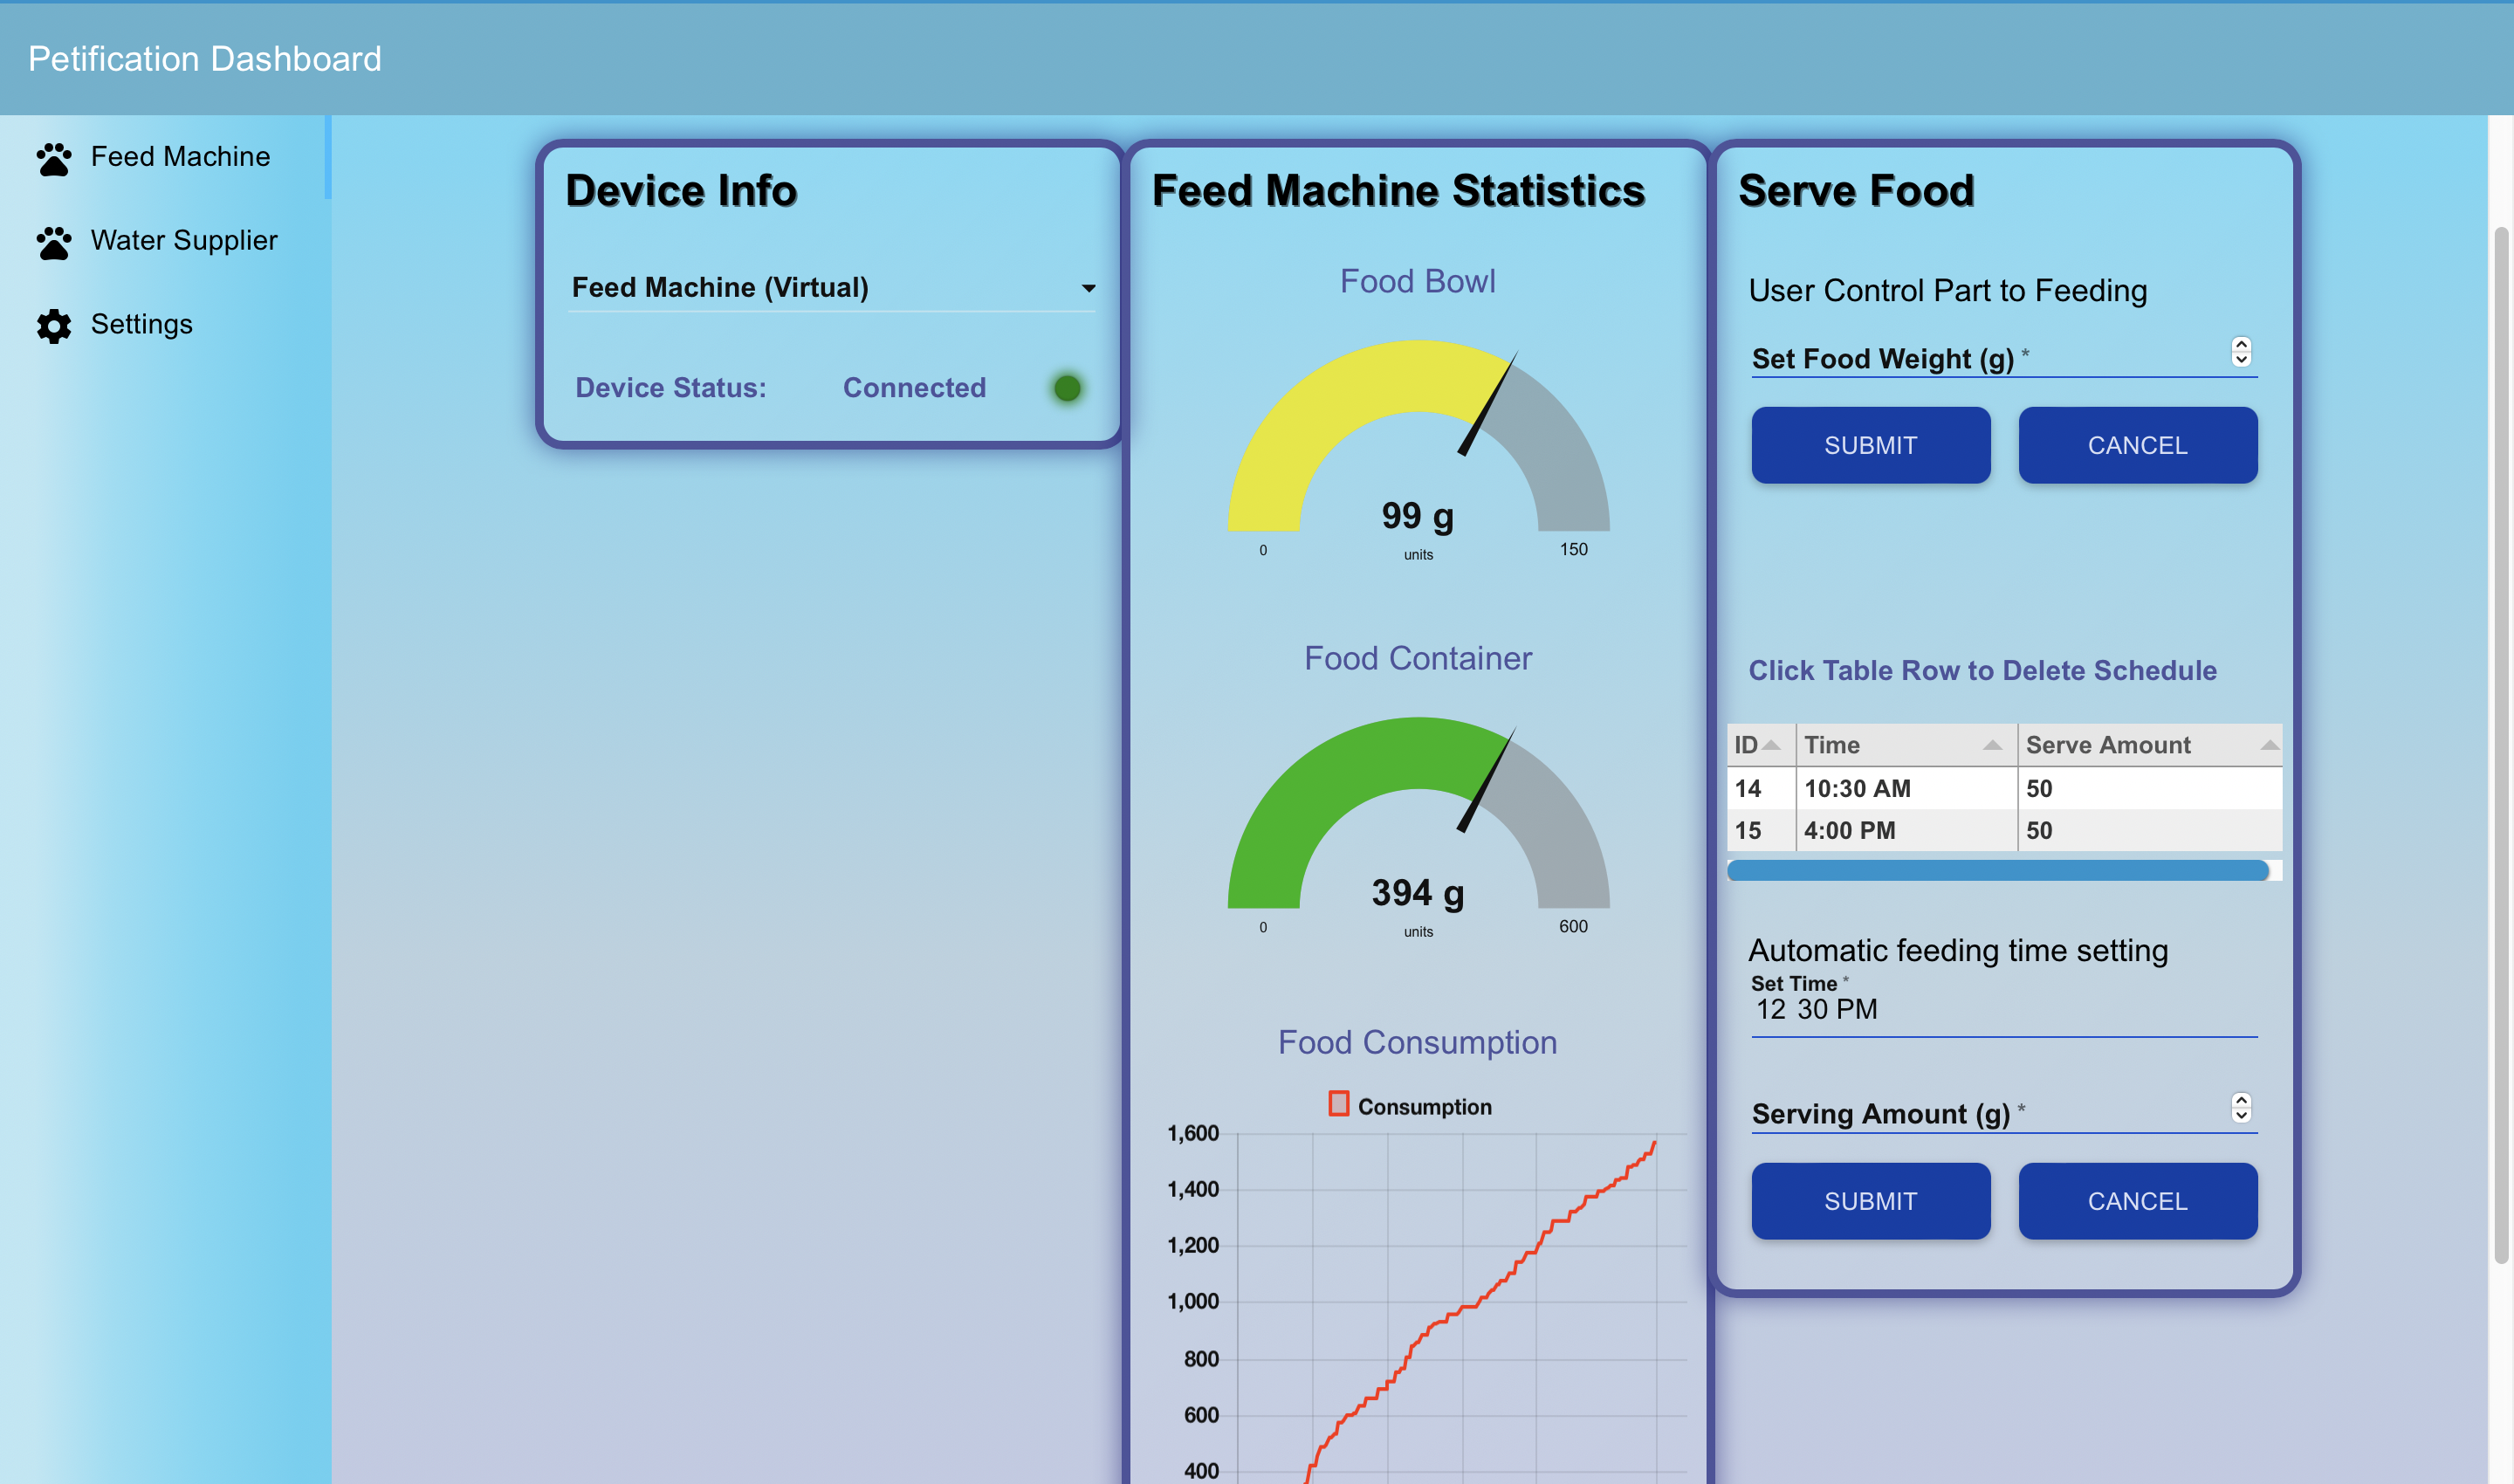
\includegraphics[width=0.5\textwidth]{./images/feed_machine_ui.png}}
\caption{Screenshot for Feed Machine tab of the dashboard}
\label{fig}
\end{figure}

\subsubsection{User Management}
The purpose of the User Manager flow is to provide a ReST API for modifying user settings.
Users can manage these 4 settings: Notification enable/disable, Email address, WhatsApp account information, and timezone where the user lives.
Also, a ReST API for sending email and WhatsApp notifications is included in this flow using the "email" node of the "node-red-node-email" node module and the "whatsapp-bot" node of the "node-red-contrib-whatsappbot" node module.

\subsubsection{Schedule Engine}
Handling and executing schedules are the main functionalities of this flow.
Every minute, the schedule engine checks the schedule table of the database and executes the actions that are scheduled to be activated at that time.
Similar to the rule engine, each action corresponding to the schedule is defined in the ReST API format, and an HTTP request is sent when the action is executed.

\subsubsection{Time-series Manager}
Managing the time-series data table of the database is the main purpose of the Time-series Manager flow.
As all the published MQTT messages are stored in a time-series data table, other flows such as dashboard flow can get and utilize the time-series data.

\section{Experiment and Testing}
Testing is conducted based on the results of the implementation.
Testing is conducted only on quantitatively verifiable results, which is accuracy testing of the food serving feature.
A total of 10 tests were performed and the desired serving amount is compared with the actual serving amount in each test.

\begin{figure}[htbp]
\centerline{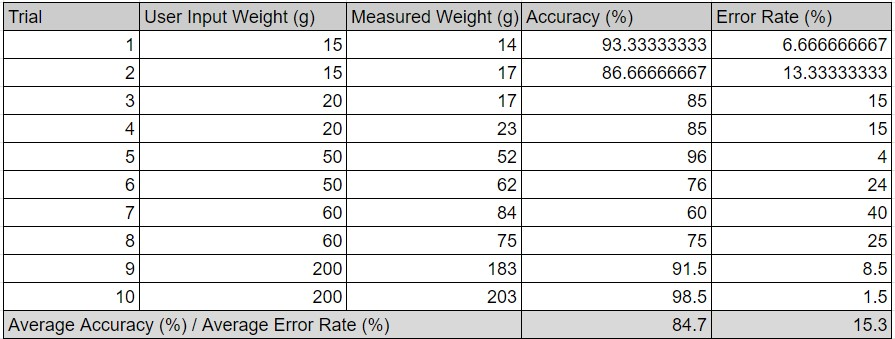
\includegraphics[width=0.5\textwidth]{./images/Feeding_sheet.jpg}}
\caption{Testing result of automatic feeding}
\label{fig}
\end{figure}

As a result of the test shown in figure 14, it was confirmed that 40\% of the highest error was found, and 1.5\% of the lowest error was found.
The reason for the error is that the food is often stuck in front of the food gate and the food serving speed is too fast for the load cell to detect.
It is a limitation for the feed machine and can be solved if the design is modified correctly.

\section{Conclusion}
In the present research, a pet-care IoT solution named "Petification" is proposed to take care of users’ pets when they are not at home.
The IoT platform for Petification is implemented using Node-RED and Eclipse Mosquitto MQTT message broker to take advantage of open-source.
The water supplier is supported in the Petification to supply water to the pet and report the current amount of the remaining water.
The feed machine is also supported to serve a certain amount of food to the pet and report the current amount of the remaining food.
The web-based dashboard is supported to allow the user to keep track of the remaining amount, consumption, and connectivity for each device.
Users can also get the notification for the emptiness of each device via email and WhatsApp messenger.
While all other functionalities are working correctly, the accuracy of serving the exact amount of food to the pet is relatively low.
The future plan can be to enhance the design of the food gate and the sensitivity and stability of the load cell to serve the exact amount of food.
Also, attaching another type of device such as a device for taking pictures of the pet can be a possible improvement for Petification.

\section{Acknowledgement}
“This research was supported by the MSIT(Ministry of Science and ICT), Korea, under the National Program for Excellence in SW) supervised by the IITP(Institute of Information \& communications Technology Planing \& Evaluation) in 2021”(2021-0-01435)
The authors of this study are grateful to Professor Minsun Lee of Chungnam National University, Professor Eric T. Matson, Professor Anthony H. Smith, and Teaching Assistant Minji Lee of Purdue University for helping us participate in the project.

\begin{thebibliography}{00}
\bibitem{b1} 
M.  Hanson.  “Pet  Industry  Statistics”  spots.com.  https://spots.com/pet-industry-statistics/ (accessed Jan. 25, 2022). 
\bibitem{b2}
Accessed: Feb. 1, 2022. [Online]. Available: https://www.instructables.com/IOT-Pet-Feeder-Using-the-Blynk-Mobile-App-an-ESP82/
\bibitem{b3}
T. Sangvanloy and K. Sookhanaphibarn, "Automatic Pet Food Dispenser by using Internet of Things (IoT)," 2020 IEEE 2nd Global Conference on Life Sciences and Technologies (LifeTech), Kyoto, Japan, Mar. 10-12, 2020.
\bibitem{b4}
Y. Chen and M. Elshakankiri, "Implementation of an IoT based Pet Care System," 2020 Fifth International Conference on Fog and Mobile Edge Computing (FMEC), Paris, France, Apr. 20-23, 2020.
\bibitem{b5}
Accessed: Feb. 4, 2022. [Online]. Available: https://iotdesignpro.com/projects/google-assistant-controlled-iot-pet-feeder-using-esp8266
\bibitem{b6}
Accessed: Feb. 5, 2022. [Online]. Available: https://create.arduino.cc/projecthub/circuito-io-team/iot-pet-feeder-10a4f3
\bibitem{b7}
Node-RED [Online]. Available: https://nodered.org/about/
\bibitem{b8}
MQTT [Online]. Available: https://mqtt.org
\bibitem{b9}
P. N. Vrishanka, P. Prabhakar, D. Shet and K. Rupali, "Automated Pet Feeder using IoT," 2021 IEEE International Conference on Mobile Networks and Wireless Communications (ICMNWC), Tumkur, Karnataka, India, Dec. 3-4, 2021.
\bibitem{b10}
R. Nogueira, H. Araújo and D. Prata. (Apr. 2019). Robot Chow: Automatic Animal Feeding with Intelligent Interface to Monitor Pets. International Journal of Advanced Engineering Research and Science. [Online]. Available: https://ijaers.com/detail/robot-chow-automatic-animal-feeding-with-intelligent-interface-to-monitor-pets/
\bibitem{b11}
Vania, K. Karyono and I. H. T. Nugroho, "Smart dog feeder design using wireless communication, MQTT and Android client," 2016 International Conference on Computer, Control, Informatics and its Applications (IC3INA), Tangerang, Indonesia, Oct. 3-5, 2016.
\bibitem{b12}
N. B. Kamarozaman and A. H. Awang, "IOT COVID-19 Portable Health Monitoring System using Raspberry Pi, Node-Red and ThingSpeak," 2021 IEEE Symposium on Wireless Technology \& Applications (ISWTA), Shah Alam, Malaysia, Aug. 17-17, 2021.
\bibitem{b13}
Eclipse Mosquitto [Online]. Available: https://mosquitto.org/
\bibitem{b14}
A. Tamboli, “Build Your Own IoT Platform,” in \textit{Apress}, 1st ed, 2019

\end{thebibliography}
\vspace{12pt}
\end{document}
